%TODO: make sure terms are defined the first time they are used: "qualifying constraints", "Lagrange functions" (in Algorithm 1), "cut set", and "connected" problem variables

\documentclass{article} % For LaTeX2e
\usepackage{nips14submit_e,times}
\usepackage{hyperref}
\usepackage{url}
%\documentstyle[nips14submit_09,times,art10]{article} % For LaTeX 2.09

%\usepackage{algorithm, algorithmic}
\usepackage{algorithm}
\usepackage[noend]{algorithmic}

\usepackage{amssymb, amsmath}
\usepackage{graphicx}
\usepackage{comment}

\newcommand{\RR}{\ensuremath{\mathbb{R}}}
\newcommand{\T}{\ensuremath{\top}}

\renewcommand{\leq}{\leqslant}
\renewcommand{\geq}{\geqslant}

\title{A Global Optimization Algorithm for \\ 
Sparse Mixed Membership Matrix Factorization}


\author{
Patrick Flaherty\\
Biomedical Engineering Department\\
Worcester Polytechnic Institute\\
Worcester, MA 01609 \\
\texttt{pjflaherty@wpi.edu} \\
\And
Fan Zhang \\
Biomedical Engineering \\
Worcester Polytechnic Institute\\
Worcester, MA 01609 \\
\texttt{fzhang@wpi.edu} \\
\And
Andrew C. Trapp \\
School of Business \\
Worcester Polytechnic Institute \\
Worcester, MA 01609 \\
\texttt{atrapp@wpi.edu}
}

% The \author macro works with any number of authors. There are two commands
% used to separate the names and addresses of multiple authors: \And and \AND.
%
% Using \And between authors leaves it to \LaTeX{} to determine where to break
% the lines. Using \AND forces a linebreak at that point. So, if \LaTeX{}
% puts 3 of 4 authors names on the first line, and the last on the second
% line, try using \AND instead of \And before the third author name.

\newcommand{\fix}{\marginpar{FIX}}
\newcommand{\new}{\marginpar{NEW}}

%\nipsfinalcopy % Uncomment for camera-ready version

\begin{document}

\maketitle

\begin{abstract}
Mixed membership models are popular for analyzing data sets that have
within-sample heterogeneity. Several sampling and variational inference
algorithms have been developed for mixed membership models, but they only
provide approximate, locally optimal estimates rather than globally optimal
etimates. We derive an alternating algorithm that provides a guaranteed
$\epsilon$-global optimum to a particular sparse mixed membership matrix
factorization problem using Benders decomposition and the Global OPtimization
(GOP) framework. We show empirical results on simulation data and describe
several extensions that improve the algorithm run time on larger data sets.
Finally, we show how the GOP methodology can be extended to achieve globally
optimal parameter estimates in general hierarchical Bayesian models.

\end{abstract}

\section{Introduction}\label{sec:intro}

Mixed-membership models have been used in document topic
modeling~\cite{Blei2003a}, collaborative filtering \cite{Mackey2010},
population genetics~\cite{Pritchard2000}, bioinformatics~\cite{Rogers2005}, and
social network analysis~\cite{Airoldi:2008wi}. Such models account for data
where an observed feature for a given sample is a mixture of shared, underlying
groups. These groups are called topics in document modeling, subpopulations in
population genetics, and communities in social network analysis. In
bioinformatics applications the groups are called subtypes and we adopt that
terminology here. Inference in mixed-membership models simultaneously
identifies both the underlying subtypes and the distribution over those
subtypes for each individual sample.



\begin{comment}
\subsection{Molecular Subtypes in Cancer}
Recently, it has become evident that many solid tumor samples are a
heterogeneous mixture of genetic subtypes~\cite{Gerlinger:2012fs}. The
heterogeneity is due to the presence of normal and immune cells in the biopsy
as well as multiple genetic subtypes in the cancer tissue~\cite{}. The measured
expression level for a gene in a sample is then a convex weighted combination
of the expression level in each cellular subpopulation where the weights are
the fraction of that subpopulation in the sample.


However, most tumor classification methods for cancer subtyping make an
all-or-none assumption~\cite{}. This assumption and subsequent treatment
decision can lead to mono-therapy treatment failure because a potentially
sizable fraction of the tumor is left untreated by focusing therapeutic effort
on the majority subtype~\cite{}. Therefore, there is a need for a
mixed-membership model to accurately estimate the tumor subtype distribution in
heterogeneous tumor samples.


\end{comment}

\subsection{Mixed Membership Models}

% Model structure
Continuous mixed membership statistical models have a latent Dirichlet random
variable that allows each sample to have its own distribution over subtypes and
a latent variable for the feature weights that describe each subtype. The
inferential goal is to estimate the joint posterior distribution over these
latent variables and thus obtain the distribution over subtypes for each sample
and the feature vector for each subtype.

Sampling or variational inference methods are commonly used to estimate the
posterior distribution of interest. A mean-field variational
algorithm~\cite{Blei2003a} and a collapsed Gibbs sampling algorithm have been
developed for Latent Dirichlet Allocation~\cite{Xiao2010}. Alternatively,
inference may be viewed as a particular matrix factorization
problem~\cite{Mackey2010}.

There is a tight connection between mixed membership models and matrix
factorization~\cite{Singh2008}. Non-negative matrix factorization techniques
have been used in image analysis and collaborative filtering applications
\cite{Lee1999,Mackey2010}. Topic models for document clustering have been cast
as a matrix factorization problem~\cite{Xu2003}.

The basic mixed membership model structure has been extended in various
interesting ways. A hierarchical Dirichlet prior allows one to obtain a
posterior distribution over the number of subtypes~\cite{Teh2005}. A prior on
the subtype variables allows one to impose specific sparsity constraints on the
subtypes~\cite{Kaban:2007gz,MacKay:1992ul,Taddy:2012dd}. Correlated information
may be incorporated to improve the coherence of the subtypes~\cite{Blei2006}.


\subsection{Benders Decomposition and Global OPtimization Framework} 
In many applications it is important to obtain the globally optimal solution
rather than a local or approximate solution. Recently there have been
significant advances in deterministic optimization methods for general
nonconvex optimization problems~\cite{Floudas2008, Horst2002}. Reviews describe
many deterministic strategies including: covering methods, branch and bound
methods, cutting plane methods, interval methods and others. Here, we build on
Benders decomposition and GOP to develop a cutting plane method to solve for
the $\epsilon$-global optimal solution for the sparse mixed membership matrix
factorization problem.


Benders decomposition provides a way to seperate the decision variables in an
optimization problem in such a way that alternating between solving two
optimization problems over the subsets of variables yields a global optimum
\cite{Benders1962,Geoffrion1972}. So-called ``complicating variables'' -
variables that when temporarily held fixed render the optimization problem more
tractable - are separated from other variables. Alternating between the two
optimization problems involving both sets of variables yields an algorithm that
converges to the global optimum. However, Benders decomposition was originally
limited to situations where the subproblem was a linear
program~\cite{Benders1962}.

The Global OPtimization (GOP) approach is a recent adaptation of Benders
decomposition that provides an $\epsilon$-global optimal solution to a more
general class of problems that includes mixed-integer biconvex optimization
problems~\cite{Floudas1990}. We develop an algorithm for sparse mixed
membership matrix factorization problem using the GOP framework to obtain an
$\epsilon$-global optimum solution.

We outline the general sparse mixed membership matrix factorization problem in
Section~\ref{sec:problem}. In Section~\ref{sec:approach} we describe our
approach using GOP and Benders decomposition to obtain an $\epsilon$-global
optimum solution. We show empirical results of our method on an example problem
in Section~\ref{sec:results}. Finally, we discuss extensions of our approach
for more general hierarchical models in Section~\ref{sec:stats}.


\section{Problem Statement}\label{sec:problem} 
The problem data is a matrix $y \in \RR^{M \times N}$, where the element
$y_{ji}$ is an observation of feature $j$ in sample $i$. We would like to
represent each column of $y$ as $y_i = x \theta_i$, where $x \in \RR^{M \times
K}$ is a matrix of $K$ subtype vectors and $\theta_i \in\Delta^{K-1}$ is the
$i$th sample's distribution over the $K$ subtypes. We would like $x$ to be
sparse because doing so makes interpreting the subtypes easier and often $x$ is
believed to be sparse a-priori for many interesting problems. In the specific
case of cancer subtyping, $y_{ji}$ may be a normalized gene expression
measurement for gene $j$ in sample $i$ in translational bioinformatics
applications. We cast the matrix factorization problem as

\begin{flalign}\label{eqn:opt1}
	\underset{\theta,x}{\text{minimize}}  &\  \|y-x\theta\|^2_2 \nonumber\\
	\text{subject to} &\  \|x\|_1 \leq P \\
	&\  \theta_i \in \Delta^{K-1}\  \forall i. \nonumber
\end{flalign}

Optimization problem~\eqref{eqn:opt1} can be recast as an optimization problem
with a biconvex objective and a convex domain:

\begin{flalign}\label{eqn:opt2}
	\underset{\theta,x,z}{\text{minimize}}      &\  	\|y-x\theta\|^2_2 \nonumber\\
	\text{subject to}   &\  \sum_{j=1}^M \sum_{k=1}^K z_{jk} \leq P \\
                    &\  -z_{jk} \leq x_{jk} \leq z_{jk} \ \forall j,k \nonumber\\
                    &\  \theta_i \in \Delta^{K-1}\  \forall i, z_{jk} \geq 0\  \forall (j,k).\nonumber
\end{flalign}

If either $x$ or $\theta$ is known then \eqref{eqn:opt2} reduces to a convex
optimization problem. Indeed, if $x$ is fixed, the optimization problem is a
form of constrained linear regression. If $\theta$ is fixed, we have a form of
LASSO regression.

A common approach for solving an optimization problem with a biconvex objective
function is to alternate between fixing one variable and optimizing over the
other. However, this approach only provides a local optimum~\cite{Gorski2007a}.


\section{Approach}\label{sec:approach}
We use the Global OPtimization approach to solve for $\epsilon$-global optimum
values of $x$ and $\theta$~\cite{Floudas1990,Floudas1994}. GOP is based on the
alternating decomposition approach of Benders
Decomposition~\cite{Geoffrion1972}, so we briefly review the approach of
Benders decomposition and GOP. Then we use the approach to derive an
$\epsilon$-global optimization algorithm for matrix factorization
problem~\eqref{eqn:opt2}.



\subsection{General Benders Decomposition and GOP}\label{sec:benders}
Benders decomposition partitions the decision variables of an optimization
problem in such a way that alternating between solving two simpler optimization
problems over the subsets of variables yields a global optimum
\cite{Benders1962,Geoffrion1972}. The master problem contains the so-called
``complicating variables'' -- variables that when temporarily held fixed render
the subproblem, consisting of only ``non-complicating variables,'' more
tractable. The subproblem is an implicit projection of the original
optimization problem onto only the space of complicating variables, represented
via a sequence of cutting planes. Benders decomposition algorithm alternates
between the master problem and subproblem to converge to a globally optimal
solution.

The GOP approach is a relatively recent extension of
Benders decomposition to a broad class of mixed integer nonlinear optimization
problems that can attain an $\epsilon$-global optimum solution through
convergence of tightening upper and lower bounds~\cite{Floudas1990}. We develop
an algorithm for sparse mixed membership matrix factorization problem using the
GOP framework and obtain an $\epsilon$-global optimum solution. The GOP
approach is summarized in Algorithm~\ref{alg:gop1}.


\begin{algorithm}[h]
\caption{General GOP Algorithm}
\label{alg:gop1}

\begin{algorithmic}[1]
\STATE Initialize master problem decision variables.
\REPEAT
\STATE Solve subproblem for fixed master problem decision variables to obtain an upper bound.
\STATE Select valid qualifying constraints and Lagrange functions from the current and all previous iterations.
\FOR{ each setting of subproblem variables at their upper and lower bounds }
\STATE Solve the relaxed master problem in the region defined by the qualifying constraints.
\ENDFOR
\STATE Set the current lower bound to the minimum of the all current and previous master problem solutions and update master problem decision variables.
\UNTIL{upper bound - lower bound is sufficiently small}
\end{algorithmic}

\end{algorithm}

\subsection{Partitioning the Biconvex Optimization Problem into the Master Problem and Subproblem}
We start by partitioning the problem into a master problem
and subproblem. The variable $Q$ is used later to enforce the
Lagrange function constraints passed from the subproblem to
the master problem; these constraints implicitly represent subproblem information in a compact manner.

\fbox{
\begin{minipage}[c][15em][t]{.7\textwidth}
\centering
  \textbf{Relaxed Master Problem} \\
  ($\theta$ fixed)
    \begin{flalign*}
    \underset{Q,x,z}{\text{minimize}}     &\  Q \\
    \text{subject to}   &\  \sum_{j=1}^M \sum_{k=1}^K    z_{jk} \leq P \\ 
                        &\  -z_{jk} \leq x_{jk} \leq z_{jk},\  z_{jk} \geq 0\\
						& \text{for}\  t = 1, \ldots, T
						\begin{cases}
						Q \geq L(x,\theta^{B_t}, y, \lambda^{(t)},\mu^{(t)})\big\vert^{\text{lin}}_{x^{(t)}, \theta^{(t)}} \\
						g^{(t)}_i\big\vert^{\text{lin}}_{x^{(t)}}(x) \leq 0\  \text{if}\  \theta^{B_t}_{ki} = 1\\
						g^{(t)}_i\big\vert^{\text{lin}}_{x^{(t)}}(x) \geq 0\  \text{if}\  \theta^{B_t}_{ki} = 0
						\end{cases}
\end{flalign*}
\end{minipage}
}
\fbox{
\begin{minipage}[c][15em][t]{.2\textwidth}
\centering
  \textbf{Subproblem} \\
  ($x$ fixed)
  	\vspace{3em}
    \begin{flalign*}
    \underset{\theta}{\text{minimize}}     &\  \|y-x\theta\|^2_2 \\
    \text{subject to}   &\  \theta_i^T 1_K = 1 \\
                    &\  \theta_{ki} \geq 0 
    \end{flalign*}
\end{minipage}%
}

GOP iterations are started by randomly initializing the master problem decision
variables at $x^{(0)}$. The loop counter $T$ is then set to $T=1$ and the
algorithm begins alternating between the subproblem and master problem.


The subproblem is solved in the $T$-th iteration using fixed $x^{(T-1)}$ from
the previous iteration of the master problem. The optimal Lagrange variables are
$\lambda^{(T)}$ and $\mu^{(T)}$ for the equality and inequality constraints.
Update the upper bound, $\text{SUBD}$, using the subproblem optimal value,
$S^{(T)}$, according to $SUBD = \min\{SUBD, S^{(T)} \}$.


\looseness-1 Information is passed from the subproblem to the master problem
through the subproblem Lagrange function, $L$ and associated qualifying
constraints, $g$. For each of the previous iterations $t=1, \ldots, T-1$, the
set of active qualifying constraints is identified at $x^{(T-1)}$ by
considering combinations with $\theta^{B_t}_{ki}$ at zero or one -- its upper
and lower bounds. All the qualifying constraints will be valid at exactly one
setting of $\theta^{B_t}$. The qualifying constraints define a cut set region
that contains $x^{(T-1)}$ - the fixed value of $x$ that yielded the current
solution of the subproblem. It is possible that the $ki$-th qualifying
constraint is not unique. In that case, the cutting plane of the equivalent
qualifying constraints overlap and we would merely solve more relaxed master
problems than necessary. The corresponding Lagrange function
$L(x,\theta^{B_t},y,\lambda^{(t)},\mu^{(t)})\big\vert^{\text{lin}}_{x^{(t)},
\theta^{(t)}}$ provides a lower bound on $Q$ in the master problem.


%By incorporating the qualifying constraints and Lagrange
%functions from \textit{all} previous iterations, the master
%solution space is sequentially tightened. Importantly, GOP
%does not require that the partitions from each iteration be
%nested, only that we look back to all of the previous
%iterations to select the appropriate qualifying constraints.

The solution space of the original optimization problem is progressively
constructed by incorporating the qualifying constraints and Lagrange functions
from \textit{all} previous iterations into the master problem. Importantly, GOP
does not require that the partitions from each iteration be nested, only that
we look back to all of the previous iterations to select the appropriate
qualifying constraints.


We briefly provide derivations for the Lagrange function and the qualifying constraints here. First, the Lagrange function for the subproblem is 
\begin{equation}\label{eqn:lagrange1}
    \begin{split}
    L(x, \theta, \lambda, \mu) &= \sum_{i=1}^N L(x, \theta_i, \lambda_i, \mu_i)\\
    &= \sum_{i=1}^N (y_i - x \theta_i)^\T (y_i - x\theta_i) - \lambda_i (\theta_i^\T 1_K - 1) - \mu_i^\T \theta_i\\
    &= \sum_{i=1}^N y_i^\T y_i -2 y_i^\T x \theta_i + \theta_i^\T x^\T x \theta_i - \lambda_i (\theta_i^\T 1_K - 1) - \mu_i^\T \theta_i
    \end{split}
\end{equation}
where $\mu \in \RR_+^{K \times N}$ and $\lambda \in \RR^N$.

The relaxed master problem makes use of the Lagrange function
linearized about $\theta^{(t)}$ which we obtain with a Taylor
series approximation,

\begin{equation}
    L(x, \theta_i, \lambda_i, \mu_i) \big\vert_{\theta^{(t)}}^{\text{lin}} \triangleq L(x, \theta_i^{(t)}, \lambda_i^{(t)}, \mu_i^{(t)}) + \sum_{k=1}^K g_{ki}^{(t)}(x) \cdot \left(\theta_{ki} - \theta_{ki}^{(t)} \right),
\end{equation}
where 
\begin{equation}\label{eqn:qc1}
g^{(t)}_{i}(x) \triangleq \nabla_{\theta_i} L \left(\theta_i, x, \lambda_i^{(t)}, \mu_i^{(t)} \right) \big\vert_{\theta_i^{(t)}} = -2 y_i^\T x + 2 \theta^{(t)\T}_i x^\T x - 1_K^\T \lambda_i^{(k)} - \mu_i^{(k)\T}.
\end{equation}

The qualifying constraint is quadratic in $x$. However, we require it to be
linear in $x$ to yield a convex domain if $g^{(t)}_{i}(x) \geq 0$ or
$g^{(t)}_{i}(x) \leq 0$. So, we linearize the Lagrangian first with respect to
$x$ at $x^{(t)}$ then with respect to $\theta_i$ at $\theta_i^{(t)}$. While the
linearized Lagrangian is not a lower bound everywhere in $x$, it is a valid
lower bound in the region bound by the qualifying constraints with $\theta_i$
set at the corresponding bounds in the Lagrange function.


The Lagrange function linearized about $x^{(t)}$ is
\begin{equation}
L(y_i, \theta_i, x, \lambda_i, \mu_i) \bigg\vert^{\text{lin}}_{x^{(t)}} \triangleq 
y_i^\T y_i - \theta_i^\T x^{(t)\T} x^{(t)} \theta_i - 2 y_i^\T x \theta_i + 2 \theta_i^\T x^{(t)\T} x \theta_i - \lambda_i(\theta_i^\T 1_K - 1) - \mu_i^\T \theta_i.
\end{equation}

Now, the Lagrange function linearized about $(x^{(t)}, \theta_i^{(t)})$ is

\begin{equation}
\begin{split}
L(y_i, \theta_i, x, \lambda_i, \mu_i) \bigg|^{\text{lin}}_{x^{(t)}, \theta_i^{(t)}} \triangleq\ & y_i^\T y_i + \theta_i^{(t)\T} x^{(t)\T} x^{(t)} \theta_i^{(t)} -2 \theta_i^{(t)\T} x^{(t)\T} x^{(t)} \theta_i \\
& - \lambda_i(1_K^\T \theta_i - 1) - \mu_i^\T \theta_i \\
& - 2 \theta_i^{(t)\T} x^\T x^{(t)} \theta_i^{(t)\T} - 2 y_i^\T x \theta_i + 2 \theta_i^{(t)\T} (x^{(t)\T} x + x^\T x^{(t)}) \theta_i
\end{split},
\end{equation}
and the gradient used in the qualifying constraint is

\begin{equation}
	\begin{split}
		g^{(t)}_i\big\vert^{\text{lin}}_{x^{(t)}}(x) &\triangleq \nabla_{\theta_i} \left[ L(y_i, \theta_i, x, \lambda_i, \mu_i) \bigg|^{\text{lin}}_{x_0} \right] \bigg|_{\theta_i^{(t)}} \\
		& = -2 x^{(t)\T} x^{(t)} \theta_i^{(t)} -2 x^\T y_i + 2 (x^{(t)\T} x + x^\T x^{(t)}) \theta_i^{(t)} - \lambda_i 1_K - \mu_i.
\end{split}
\end{equation}

Once the valid qualifying constraints from the previous
$t=1,\ldots,T-1$ iterations have been identified and
incorporated, the constraint for the current $T$-th iteration
is

\begin{eqnarray*}
Q \geq & L(x,\theta^{B_T}, y, \lambda^{(t)},\mu^{(t)})\big\vert^{\text{lin}}_{x^{(t)}, \theta^{(t)}}\\
&g_{ki}^{(T)}\big\vert^{\text{lin}}_{x^{(t)}}(x) \leq 0 \ \text{if}\ \theta^{B_T}_{ki} = 1 \\
&g_{ki}^{(T)}\big\vert^{\text{lin}}_{x^{(t)}}(x) \geq 0 \ \text{if}\ \theta^{B_T}_{ki} = 0.
\end{eqnarray*}
The master problem must be solved once for each possible setting of the
subproblem variables at their bounds. In general, we only need to set the
``connected'' subproblem variables at their bounds, but the matrix
factorization problem structure renders all $KN$ subproblem variables
connected. Thus we have the computationally complex situation of needing to
solve $2^{KN}$ relaxed master problems at each iteration. This is the price we
pay for an exact solution. However, as detailed later, there are several ways
of reducing this computational burden.

All of the $2^{KN}$ solutions, $Q$, of the relaxed master problem are appended
to a list at each iteration. The minimum $Q$ in this list is selected for the
new global lower bound $\text{MLBD}$ and the optimal $x^{(T)}$ is updated to
the corresponding optimizing decision variable. The solution is removed from
the list so that it is not selected in a later iteration. If the lower and
upper bounds are within the specified tolerance $\epsilon$, the algorithm
terminates with the $\epsilon$-global optimum solution in $x^{(T)}$. Finite
$\epsilon$-convergence and $\epsilon$-global optimality proofs are given
in~\cite{Floudas1994}.

\section{Experiments}\label{sec:results}

We use a simple data set in order to show the
operation of the algorithm in detail and facilitate visualization of the cut sets. The data set, $y$, and true
decision variable values, $(x^*, \theta^*)$, are

\begin{eqnarray*}
	x^* =
	\left[ 
	\begin{array}{cc} 
		-1, & 0
	\end{array} 
	\right],
	&
	\theta^* = 
	\left[ 
	\begin{array}{ccc} 
		1, & 0, & 0.5 \\
		0, & 1, & 0.5
	\end{array} 
	\right],
	&
	y = 
	\left[ 
	\begin{array}{ccc} 
		-1, & 0, & -0.5
	\end{array} 
	\right].
\end{eqnarray*}
Note that the optimal objective function value is zero.

We ran the GOP algorithm with sparsity constraint variable $P=1$ and
convergence tolerance $\epsilon = 0.01$. There are $KN = 6$ connected
variables, so we solve $2^{KN} = 64$ relaxed master problems at each iteration.
These relaxed master problems are independent and can be distributed to
different computational threads or cores. The subproblem is a single
optimization problem and need not be distributed. The optimal decision
variables after 73 iterations are

\begin{eqnarray*}
	\hat{x} = x^{(73)} =
	\left[ 
	\begin{array}{cc} 
		-0.920, & 0.080
	\end{array} 
	\right],
	&
	\hat{\theta} = \theta^{(73)} =
	\left[ 
	\begin{array}{ccc} 
		1.00, & 0.080, & 0.580 \\
		0.00, & 0.920, & 0.420
	\end{array} 
	\right],
\end{eqnarray*}
and the Lagrange multipliers are $\hat{\lambda} = [-0.147, 0, 0]$ and $\hat{\mu} = [0, 0, 0; 0.160, 0, 0]$.

Figure~\ref{fig:figs_bounds_and_trace}A shows the convergence of the upper and
lower bounds by iteration. The upper bound converges quickly and the majority
of the time in the algorithm is spent proving optimality. With each iteration
regions of the solution space are tested until the lower bound is tightened
sufficiently to meet the stopping criterion.

Figure~\ref{fig:figs_bounds_and_trace}B shows the first six $x$ values
considered by the algorithm with isoclines of the objective function with
$\theta^*$ fixed. It is evident that the algorithm is not performing
hill-climbing or any other gradient ascent algorithm during its search for the
global optimum. Instead, the algorithm explores a region bound by the
qualifying constraints to construct a lower bound on the objective function.
Furthermore, the algorithm does not search nested regions, but considers
previously explored cut sets.

\begin{figure}[ht]
	\centering
		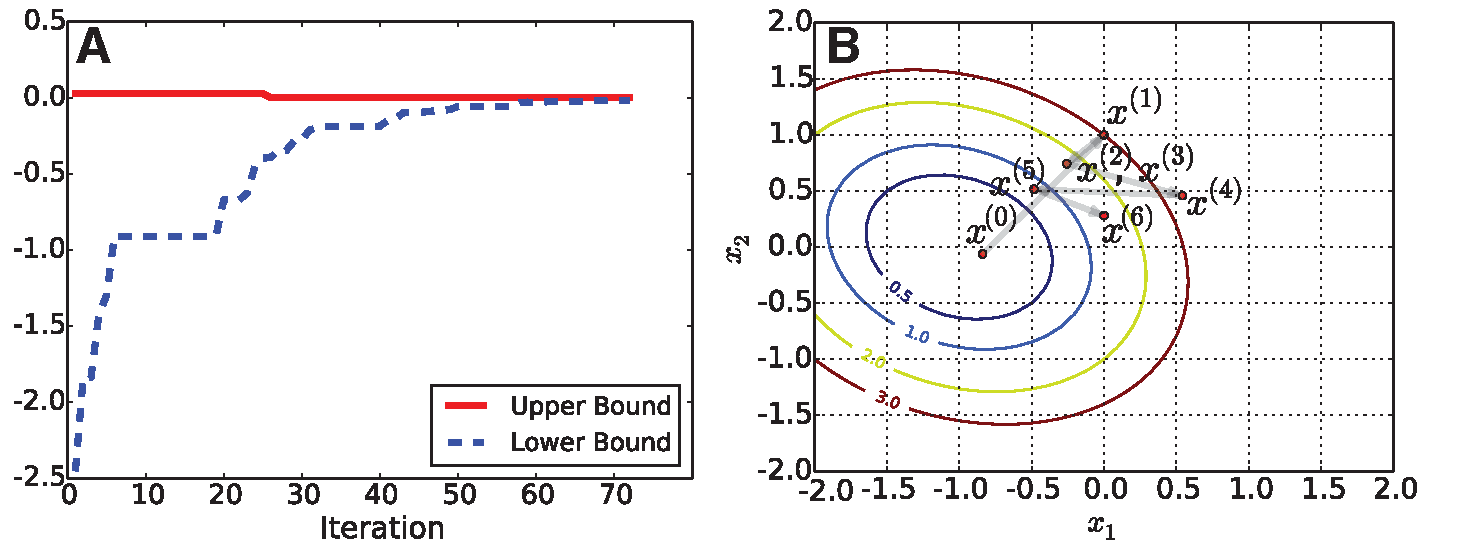
\includegraphics[width=1.0\textwidth]{figs/bounds_and_trace.pdf}
	\caption{(A) Upper and lower bounds converge to $\epsilon$-global optimal solution. (B) First six iterations of GOP algorithm in $x$ space with contours of the objective function at optimal $\theta^*$.}
	\label{fig:figs_bounds_and_trace}
\end{figure}

Figure~\ref{fig:figs_GOP_cutting_plane_sequence} shows the sequence of cut sets
for the first three iterations of the algorithm. One cutting plane is obtained
for each of the $KN$ qualifying constraints. We initialize the algorithm at
$x^{(0)}$. The blue solid lines in the subfigure for the zero-th iteration show
the cuts with $g^{(t)}_i\big\vert^{\text{lin}}_{x^{(t)}}(x) = 0$. The GOP
algorithm solves $2^{KN}$ relaxed master problems to provide a lower bound in
each region. The value of $x$ that yields the smallest lower bound is selected
for the next iteration -- shown as $x^{(1)}$. There are $KN=6$ cuts, but only
five are visible in the figure becasue two of the cuts overlap. Then $KN$ cuts
are generated about $x^{(1)}$ (shown in the middle subfigure). The previous
cuts are shown as dotted lines. Again $2^{KN}$ relaxed master problems are
solved, but now the regions are the intersecton of the region containing
$x^{(1)}$ from the previous iteration and all of the regions defined in the
current iteration cut set. The $x$ that achieves the lowest lower bound is
selected as $x^{(2)}$ and the algorithm continues incorporating the previous
cut regions.


\begin{figure}[ht]
	\centering
		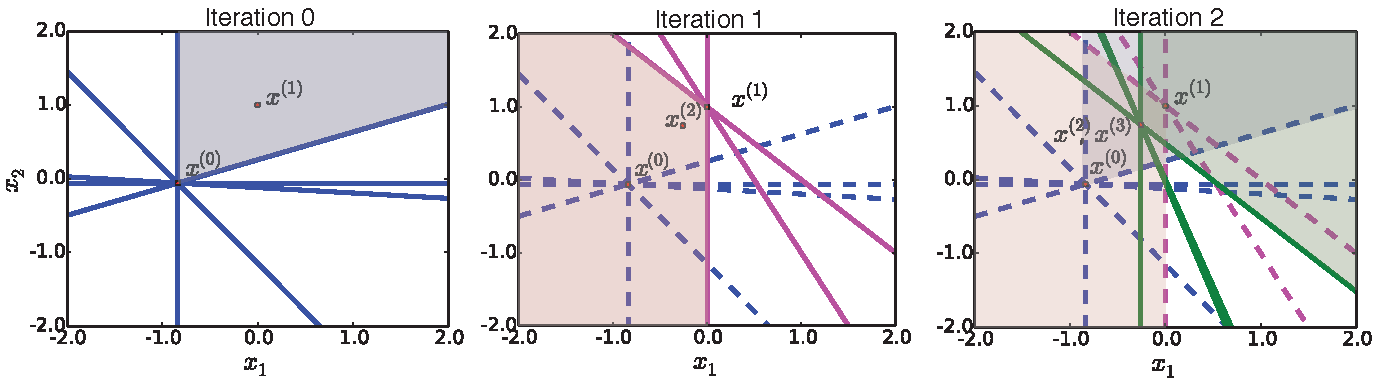
\includegraphics[width=1.0\textwidth]{figs/GOP_cutting_plane_sequence.pdf}
	\caption{Cut set regions for the first three iterations of the GOP algorithm for sparse mixed membership matrix factorization. Refinement of the relaxed master problem solution space and lower bound achieves $\epsilon$-global optimality.}
	\label{fig:figs_GOP_cutting_plane_sequence}
\end{figure}

\section{Extensions of GOP for Hierarchical Models}\label{sec:stats}

The general scalar exponential family distribution function takes the form
\begin{equation}
	f_X(x|\eta) = h(x)\exp\left\{ \eta T(x) - A_X(\eta) \right\},
\end{equation}
where $\eta$ is the natural parameter, $T(x)$ is the sufficient statistic, $h(x)$ is the base measure, and $A(\eta)$ is the log-partition function.

Consider a hierarchical Bayesian model with a prior on $\eta$ with hyperparameters $\nu$,
\begin{equation}
	f_\eta(\eta|\nu) = h(\eta)\exp\left\{ \nu T(\eta) - A_\eta(\nu) \right\},
\end{equation}

The joint distribution is then
\begin{equation}\label{eqn:joint_exp}
	f_{(X,\eta)}(x,\eta | \nu) = h(x)h(\eta)\exp\left\{ \eta T(x) + \nu T(\eta) - A_X(\eta) -A_\eta(\nu)\right\}.
\end{equation}

If $\eta$ was known then the maximum likelihood estimate (MLE) for $\nu$ could be found by setting the derivative of \eqref{eqn:joint_exp} with respect to $\nu$ to zero and solving for $\eta$. Similarly, if $\nu$ was known, we could solve for $\eta$ by the same procedure. However, since both are unknown the MLE must be found as
\begin{flalign}\label{eqn:gen_mod_opt}
	\underset{\eta, \nu}{\text{minimize}}  &\  - \log f_{(X,\eta)}(x,\eta | \nu) \nonumber \\
	\text{subject to} &\  G(\eta, \nu) \leq 0 \\
	&\  H(\eta, \nu) = 0, \nonumber \\
\end{flalign}
where we have written the MLE problem as a standard minimization problem.

GOP requires the following general conditions on $f_{(X,\eta)}(x, \eta | \nu)$:
\begin{enumerate}
	\item $-\log f_{(X,\eta)}(x, \eta | \nu)$ is convex in $\eta$ for every fixed $\nu$, and convex in $\nu$ for every fixed $\eta$,
	\item $G(\eta,\nu)$ is convex in $\eta$ for every fixed $\nu$, and convex in $\nu$ for every fixed $\eta$,
	\item $H(\eta, \nu)$ is affine in $\eta$ for every fixed $\nu$, and affine in $\nu$ for every fixed $\eta$,
	\item Appropriate first-order constraint qualifications are satisfied (e.g. Slater's constraint qualification).
\end{enumerate}

Conditions 2-4 are satisfied for general hierarchical models. Condition 1 is satisfied for $\nu$ because $\frac{\partial^2 - \log f_{(X,\eta)}(x,\eta | \nu)}{\partial \nu^2} = \frac{\partial^2 A_\eta(\nu)}{\partial \nu^2}$, and $A_\eta(\nu)$ is convex. Condition 1 is satisfied when
\begin{equation}
	\frac{\partial^2 - \log f_{(X,\eta)}(x,\eta | \nu)}{\partial \eta^2} = -\nu \frac{\partial^2 T(\eta)}{\partial \eta^2} + \frac{\partial^2 A_X(\eta)}{\partial \eta^2} - \frac{\partial^2 \log h(\eta)}{\partial \eta^2} \geq 0.
\end{equation}

So we have the condition
\begin{equation}
	\frac{\partial^2 A_X(\eta)}{\partial \eta^2} \geq \nu \frac{\partial^2 T(\eta)}{\partial \eta^2} + \frac{\partial^2 \log h(\eta)}{\partial \eta^2},
\end{equation}
which is satisfied when $\nu \geq 0$ and both $T(\eta)$ and $\log
h(\eta)$ are concave or when $T(\eta)$ and $\log h(\eta)$ are affine.


Then one can use Benders decomposition to separate the two
decision variables, here the latent variables and
hyper-parameters, into the master and subproblems
and derive an algorithm for the $\epsilon$-global optimal latent
variables and hyper-parameters that maximize the joint distribution.

\section{Discussion}

The main computational cost of GOP-based algorithms is the need to solve
multiple relaxed master problems at each iteration. Many of these problems are
redundant or yield optimal solutions that are greater than the current upper
bound and thus not useful. A branch-and-bound framework~\cite{Floudas1994}
combined with a mixed-integer linear program to search for the minimum lower
bound at each iteration reduces the need to solve all possible relaxed master
problems by fathoming parts of the solution space. We have implemented this
approach. In limited testing, the average time per iteration is greatly reduced
and the algorithm converges in 8 iterations rather than 73 iterations for the
cutting plane method for the example data set.

We have derived an algorithm for particular loss functions for the sparsity
constraint and objective function. However, the GOP framework can handle a
broader class of problems. We require only that the master problem and
subproblem space be compact convex sets. So other loss functions for the
sparsity constraint may be considered. Structured sparsity constraints can be
defined and incorporated in a similar way as for elastic-net regression. It may
be useful to consider other loss functions for the objective function depending
on the application.

We are exploring the connections between GOP and the other alternating
optimization algorithms such as the EM and variational EM algorithm. Since the
complexity of GOP only depends on the connected variables, the graphical model
structure connecting the master and subproblem variables may be used to
identify the worst-case complexity of the algorithm prior to running the
algorithm. A factorized graph structure may provide an approximate, but
computationally efficient algorithm based on GOP. Additionally, because the
Lagrange function factorizes into the sum of Lagrange functions for each sample
in the data set, we may be able to update the parameters based on GOP for a
selected subset of the data in an iterative or sequential algorithm. We are
exploring the statistical consistency properties of such an update procedure.

\begin{comment}
	
\subsubsection*{Acknowledgments}

Use unnumbered third level headings for the acknowledgments. All
acknowledgments go at the end of the paper. Do not include acknowledgments in
the anonymized submission, only in the final paper.
 

\end{comment}

\begin{comment}

\section*{Appendix}
\appendix
\section{Derivation of Relaxed Master Problem Constraints}

The Lagrange function is the sum of the Lagrange functions for each sample,
\begin{equation}
L(y, \theta, x, \lambda) = \sum_{i=1}^n L(y_i, \theta_i, x, \lambda_i, \mu_i),
\end{equation}
and the Lagrange function for a single sample is
\begin{equation}
L(y_i, \theta_i, x, \lambda_i, \mu_i) = y_i^T y_i -2 y_i^T x\theta_i + \theta_i^T x^T x \theta_i - \lambda_i(\theta_i^T 1_K - 1) -\mu_i^T \theta_i.
\end{equation}

We see that the Lagrange function is biconvex in $x$ and $\theta_i$. We develop the constraints for a single sample for the remainder.

\subsection{Linearized Lagrange function with respect to $x$}

Casting $x$ as a vector and rewriting the Lagrange function gives
\begin{equation}
L(y_i, \theta_i, \bar{x}, \lambda_i, \mu_i) = a_i - 2b_i^T\bar{x} + \bar{x}^TC_i\bar{x} - \lambda_i(\theta_i^T 1_K - 1) -\mu_i^T\theta_i,
\end{equation}
where $\bar{x}$ is formed by stacking the columns of $x$ in order. The coefficients are formed such that
\begin{eqnarray*}
a                     &=&    y_i^T y_i, \\
b_i^T \bar{x}         &=& y_i^T x \theta_i, \\
\bar{x}^T C_i \bar{x} &=& \theta_i^T x^T x \theta_i.
\end{eqnarray*}

The linear coefficient matrix is the $KM \times 1$ vector,
\begin{equation*}
b_i = \left[ y_{i}\theta_{1i}, \cdots, y_{i}\theta_{Ki} \right]
\end{equation*}


The quadratic coefficient is the $KM \times KM$ and block matrix
\begin{equation*}
C_i = 
\left[
\begin{array}{ccc}
\theta^2_{1i} I_M & \cdots & \theta_{1i} \theta_{Ki} I_M \\
\vdots & \ddots & \vdots \\
\theta_{Ki} \theta_{1i} I_M & \cdots & \theta^2_{Ki} I_M 
\end{array} 
\right]
\end{equation*}

The Taylor series approximation about $x_0$ is
\begin{equation}
 L(y_i, \theta_i, \bar{x}, \lambda_i, \mu_i) \bigg|^{\text{lin}}_{\bar{x}_0} = L(y_i, x_0, \theta_i, \lambda_i, \mu_i) + (\nabla_x L \big|_{x_0})^T(x-x_0).
\end{equation}

The gradient with respect to $x$ is
\begin{equation}
\nabla_x L(y_i, \theta_i, \bar{x}, \lambda_i, \mu_i) = -2 b_i + 2 C_i \bar{x}.
\end{equation}

Plugging the gradient into the Taylor series approximation gives
\begin{equation}
L(y_i, \theta_i, \bar{x}, \lambda_i) \bigg|^{\text{lin}}_{\bar{x}_0} = a_i - 2b_i^T\bar{x}_0 + \bar{x}_0^TC_i\bar{x}_0 - \lambda_i(\theta_i^T 1_K - 1) - \mu_i^T \theta_i + (-2 b_i + 2 C_i \bar{x}_0)^T(\bar{x}-\bar{x}_0).
\end{equation}

Simplifying the linearized Lagrange function gives
\begin{equation}\label{eqn:lagrange_linx}
L(y_i, \theta_i, \bar{x}, \lambda_i, \mu_i) \bigg|^{\text{lin}}_{\bar{x}_0} = (y_i^T y_i - \bar{x}_0^T C_i \bar{x}_0 - \lambda_i(\theta_i^T 1_K - 1) - \mu_i^T \theta_i) - 2 b_i^T \bar{x} + 2 \bar{x}_0^T C_i \bar{x}
\end{equation}

Finally, we write the linearized Lagrangian using the matrix form of $x_0$,

\begin{equation}
L(y_i, \theta_i, x, \lambda_i, \mu_i) \bigg|^{\text{lin}}_{x_0} = 
y_i^T y_i^T - \theta_i^T x_0^T x_0 \theta_i - 2 y_i^T x \theta_i + 2 \theta_i^T x_0^T x \theta_i - \lambda_i(\theta_i^T 1_K - 1) - \mu_i^T \theta_i
\end{equation}

While the original Lagrange function is convex in $\theta_i$ for a fixed $x$, the linearized Lagrange function is not necessarily convex in $\theta_i$. This can be seen by collecting the quadratic, linear and constant terms with respect to $\theta_i$,

\begin{equation}
L(y_i, \theta_i, x, \lambda_i, \mu_i) \bigg|^{\text{lin}}_{x_0} = 
(y_i^T y_i^T + \lambda_i) + (- 2 y_i^T x -\lambda_i 1_K^T -\mu_i^T ) \theta_i + \theta_i^T (2 x_0^T x - x_0^T x_0 ) \theta_i.
\end{equation}

Now, if and only if $2x_0^Tx - x_0^Tx_0 \succeq 0$ is positive semidefinite, then $L(y_i, \theta_i, x, \lambda_i, \mu_i) \bigg|^{\text{lin}}_{x_0}$ is convex. The condition is satisfied at $x = x_0$ but may be violated at some other value of $x$. 

\textbf{Can we add a LMI constraint to the relaxed master problem to ensure that the function is convex and the linearization with respect to theta is a lower bound?}

\subsection{Linearized Lagrange function with respect to $\theta_i$}
Now, we linearize \eqref{eqn:lagrange_linx} with respect to $\theta_i$. Using the Taylor series approximation with respect to $\theta_{0i}$ gives

\begin{equation}
L(y_i, \theta_i, x, \lambda_i, \mu_i) \bigg|^{\text{lin}}_{x_0, \theta_{0i}} = L(y_i, \theta_{0i}, x, \lambda_i, \mu_i) \bigg|^{\text{lin}}_{x_0} + \left( \nabla_{\theta_i} L(y_i, \theta_i, x, \lambda_i, \mu_i) \bigg|^{\text{lin}}_{x_0} \bigg|_{\theta_{0i}} \right)^T (\theta_i - \theta_{0i})
\end{equation}

The gradient for this Taylor series approximation is
\begin{equation}
g_i(x) \triangleq \nabla_{\theta_i} L(y_i, \theta_i, x, \lambda_i, \mu_i) \bigg|^{\text{lin}}_{x_0} \bigg|_{\theta_{0i}} = -2 x_0^T x_0 \theta_{0i} -2 x^T y_i + 2 (x_0^T x + x^T x_0) \theta_{0i} - \lambda_i 1_K - \mu_i,
\end{equation}
where $g_i(x)$ is the vector of $K$ qualifying constraints associated with the Lagrange function. The qualifying constraint is linear in $x$.

Plugging the gradient into the approximation gives
\begin{equation}
\begin{split}
L(y_i, \theta_i, x, \lambda_i, \mu_i) \bigg|^{\text{lin}}_{x_0, \theta_{0i}} =\ & y_i^T y_i^T - \theta_{0i}^T x_0^T x_0 \theta_{0i} - 2 y_i^T x \theta_{0i} + 2 \theta_{0i}^T x_0^T x \theta_{0i} - \lambda_i(\theta_{0i}^T 1_K - 1) - \mu_i^T \theta_{0i} \\
& + (-2 x_0^T x_0 \theta_{0i} -2 x^T y_i + 2 (x_0^T x + x^T x_0) \theta_{0i} - \lambda_i 1_K - \mu_i)^T (\theta_i - \theta_{0i})
\end{split}
\end{equation}

The linearized Lagrange function is bi-linear in $x$ and $\theta_i$.

Finally, simplifying the linearized Lagrange function gives
\begin{equation}
\begin{split}
L(y_i, \theta_i, x, \lambda_i, \mu_i) \bigg|^{\text{lin}}_{x_0, \theta_{0i}} =\ & y_i^T y_i^T + \theta_{0i}^T x_0^T x_0 \theta_{0i} -2 \theta_{0i}^T x_0^T x_0 \theta_i - \lambda_i(1_K^T \theta_i - 1) - \mu_i^T \theta_i \\
& - 2 \theta_{0i}^T x^T x_0 \theta_{0i} - 2 y_i^T x \theta_i + 2 \theta_{0i}^T (x_0^T x + x^T x_0) \theta_i
\end{split}
\end{equation}

\end{comment}

%\subsubsection*{References}
\bibliographystyle{plain}
\small
\bibliography{nips_gop}

\end{document}
